%% This is an example first chapter.  You should put chapter/appendix that you
%% write into a separate file, and add a line \include{yourfilename} to
%% main.tex, where `yourfilename.tex' is the name of the chapter/appendix file.
%% You can process specific files by typing their names in at the 
%% \files=
%% prompt when you run the file main.tex through LaTeX.
\chapter{Execution Profile of Linux Services}
This chapter first provides some background on the
Linux startup process (Section \ref{linuxboot}).  
It then describes how we collected user-level instruction
streams from some Linux services via dynamic instrumentation to 
measure nondeterminism in the linux boot process (Section \ref{datacollection});
finally, it summarizes our results on the statistical nature
of nondeterminism in Linux services (Section \ref{bootresults}).

\section{The Linux Boot Process}\label{linuxboot}
When a computer boots up:
\begin{enumerate}
\item The BIOS (Basic Input/Output System) 
gets control and performs startup tasks for the specific hardware platform.
\item Next, the BIOS reads and executes code from a designated boot device 
that contains part of a Linux boot loader. Typically,
this smaller part (or phase 1) 
loads the bulk of the boot loader code (phase 2).
\item The boot loader may present the user with options for 
which operating system to load (if there are multiple available options).
In any case, the boot loader loads and decompresses the operating system
into memory; it sets up system hardware and
memory paging; finally, it transfers control to the kernel's
\texttt{start\_kernel()} function.
\item The \texttt{start\_kernel()} function performs the 
majority of system setup (including interrupts, remaining memory
 management, device initialization)
before spawning the \texttt{idle} process, the scheduler
and the user-space \texttt{init} process.
\item The scheduler effectively takes control of system management,
and kernel stays idle unless externally called from now on.
\item The \texttt{init} process executes scripts that set up all
non-operating system services and structures in order to allow 
a user environment to be created, and then presents the user with a login screen.
\end{enumerate}

\begin{figure}[h]
  \centering
  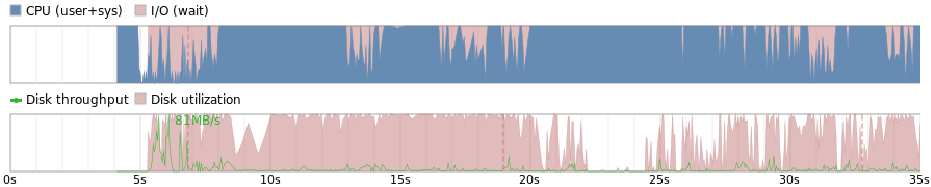
\includegraphics[width=1.04\textwidth]{boot_first35seconds.png}
  \caption[CPU and disk activity for a booting Ubuntu VM (0-35 seconds after \texttt{init} is spawned)]%
  {CPU and disk activity for a booting Ubuntu VM (0-35 seconds after \texttt{init} is spawned).
  The first few seconds show no activity because
  the data collection daemon takes a few seconds to start.}
  \label{boot:first35}
\end{figure}

\begin{figure}[h]
  \center
  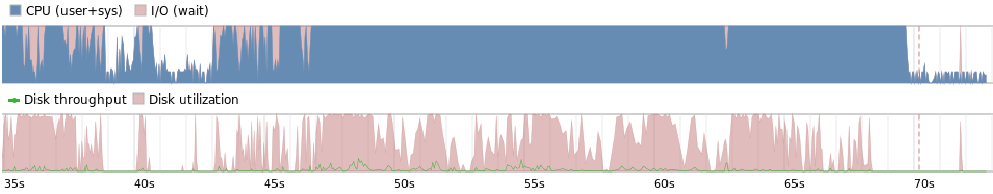
\includegraphics[width=1.10\textwidth]{boot_last35seconds.png}
  \caption[(... continued) CPU and disk activity for a booting VM (35-73 seconds after \texttt{init} is spawned) ]%
  {CPU and disk activity for a booting Ubuntu VM (35-73 seconds after \texttt{init} is spawned).}
  \label{boot:last35}
\end{figure}

Figures \ref{boot:first35} and \ref{boot:last35}
illustrate the CPU usage and disk activity 
of an Ubuntu 10.10 VM that takes about 70 seconds
to complete the sixth step of the boot process (spawning 
the \texttt{init} process to set up the user environment).
The Linux kernel version is 2.6.35-27-generic
and the VM is configured with a single core processor
with 512 Mb RAM. Generated using
the Bootchart utility \cite{mahkovec2005bootchart},
the figures illustrate that
the booting process involves high memory
and CPU overhead (5-70 seconds); they also 
show a glimpse of the well-known fact that memory and CPU
overhead typically dimishes greatly after the boot
process is completed and the machine is
ready for login (70+ seconds). This disparity
in CPU/memory usage is the source of the boot storm problem;
a single host can handle many VMs in
steady-state usage, but the host gets crippled
when the same VMs boot up concurrently.

In the last step of the booting
process (step 6), \texttt{init} typically
runs many scripts located in 
specific directories such as \texttt{`/etc/rc'}
or \texttt{`/etc/init.d/'}. While the myriad Linux distributions
can have their own variants of \texttt{init} binaries
(e.g. \texttt{SysV}, or \texttt{systemd} or \texttt{Upstart}),
the \texttt{init} process always directly/indirectly launches several 
services and daemons to initialize the user desktop
environment. Figure \ref{boot:services} provides a
summary of the specific actions performed by \texttt{init} 
(through the subprocesses or daemons it launches)
for the same Ubuntu VM used for 
Figures \ref{boot:first35} and \ref{boot:last35}.

\begin{figure}[h]
  \center
  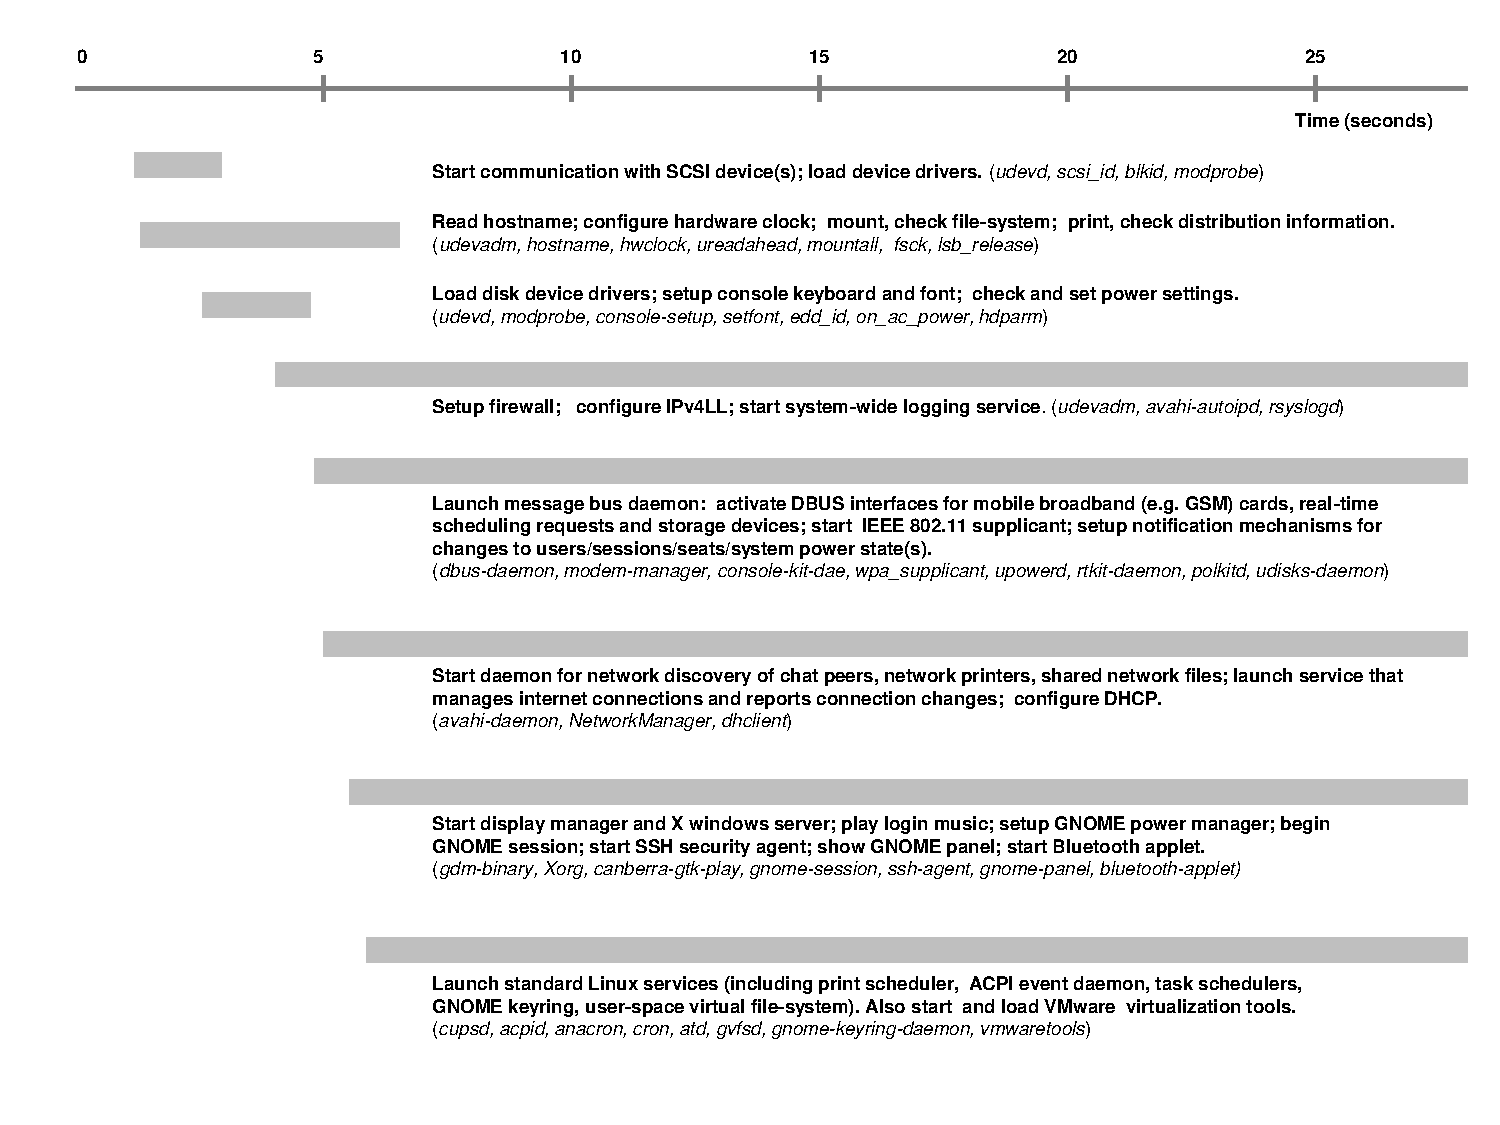
\includegraphics[width=1.0\textwidth, trim=0.5cm 1cm 1cm 1cm]{boottimeline.pdf}
  \caption[A summary of the actions performed by \texttt{init} for a booting VM]%
  {A summary of the actions performed by \texttt{init} for a booting VM;
  this figure has the same timeline (0-70 seconds) as Figures \ref{boot:first35} and 
  \ref{boot:last35}.}
  \label{boot:services}
\end{figure}

In fact, the \texttt{init} process actually launched 361 children processes (directly
and indirectly) over the 70 second period summarized by Figure \ref{boot:services}.
Most of them were ephemeral processes; several processes were repeatedly launched
in different contexts (e.g. \texttt{getty} or \texttt{grep}). The processes singled out
in Figure \ref{boot:services} are the ones that either 
stayed alive through most of the boot process till the end, performed important
boot actions, or spawned many sub-processes themselves.

\section{Data Collection Scheme} \label{datacollection}
\begin{figure}[h]
  \center
  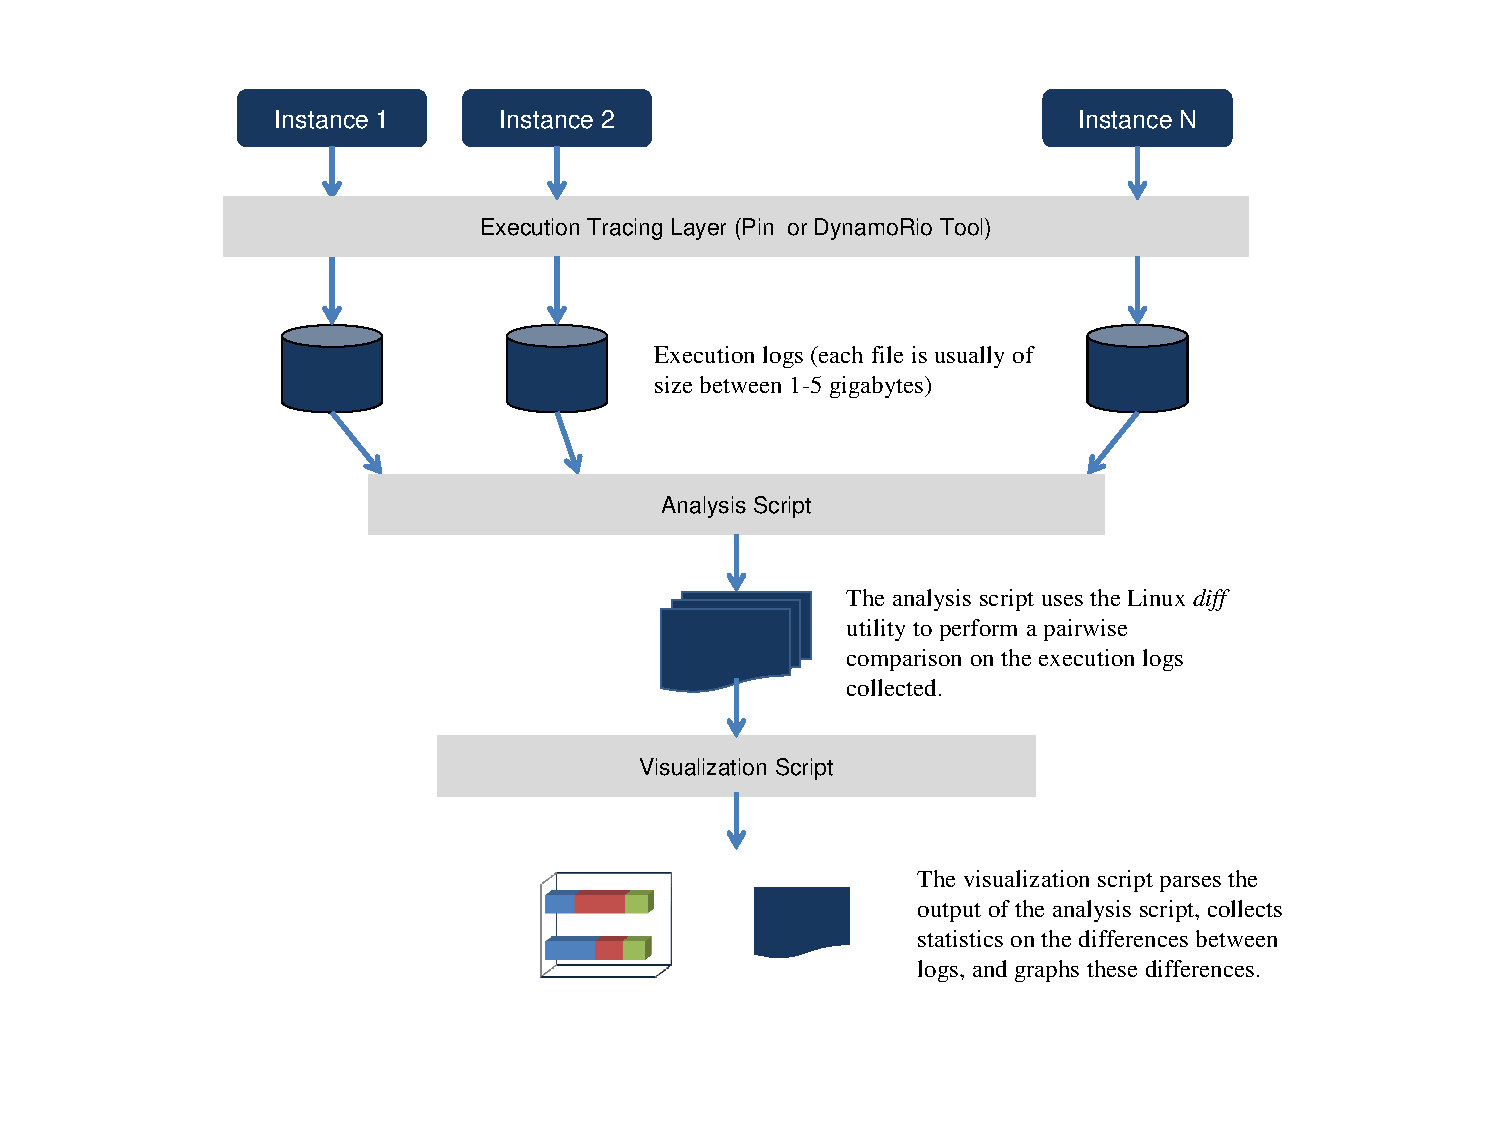
\includegraphics[width=1.0\textwidth, trim=1cm 1cm 1cm 1cm]
                  {naivedatacollection.pdf}
  \caption[Steps involved in measuring execution nondeterminism]%
  {Steps involved in measuring execution nondeterminism.}
  \label{data:naive}
\end{figure}

Pin and DynamoRio are runtime frameworks that enable inspection
and arbitrary transformation of user-mode application code as it executes.
Using both Pin and DynamoRio to study the behavior
of Linux services together allowed us to verify the
the accuracy of our results. We used Pin more 
than DynamoRio because it gets injected into application code
earlier than DynamoRio, which allows for greater
instruction coverage for our purpose.  

Figure \ref{data:naive} shows the simple steps involved
in collecting data on nondeterminism using
dynamic instrumentation. The next section 
explains each of these steps in detail, 
using a simple ``Hello, world!'' program as an example.

\subsection{Analyzing a simple ``Hello, world!'' program}
This section outlines the data collection scheme
described in Figure \ref{data:naive} in detail with the help
of an example:  the simple ``Hello, world!'' program
outlined in Figure \ref{source:hw}.
For this example, we disabled ASLR (Address Space Layout
Randomization) on the Ubuntu VM described in section \ref{linuxboot}. \newline

\begin{figure}[h]
  \lstset{frame=shadowbox, rulesepcolor=\color{black},
    basicstyle=\small, numbers=left, numberstyle=\footnotesize}
  \lstinputlisting[language=C]{helloworld.c}
  \caption[A ``Hello, world!'' program in C.]%
          {A ``Hello, world!'' program in C. }
          \label{source:hw}
\end{figure}

\noindent {\bf Execution Tracing Layer} \newline
As shown in Figure \ref{data:naive}, the first step
in data collection involves running the target program
a few times across identical VMs. Ideally, these 
different executions are done concurrently. 
In our scheme, we wrote a Pin tool that:
\begin{enumerate}
\item logs each x86 instruction executed by 
  the target process, along with the 
  new values of any affected registers, 
\item records values written to or 
  read from memory,
\item intercepts all signals received, and records the instruction counts 
  corresponding to the timing of any signals, and
\item monitors all system calls made by the target process,
  and logs any corresponding side-effects to memory or registers.
\end{enumerate}

Implementation of the execution tracing layer required
a detailed understanding and close examination of the Linux system call interface. 
Figure \ref{hw:logsys} shows an excerpt from a trace file
generated by our Pin tool while running the ``Hello, World'' 
program. Our tool records and analyzes
every instruction executed in user-space by the process
for the ``Hello, world'' program once Pin gets control; 
this allows us to include program initialization
and library code in our analysis.

\begin{figure}[h]
  \center
  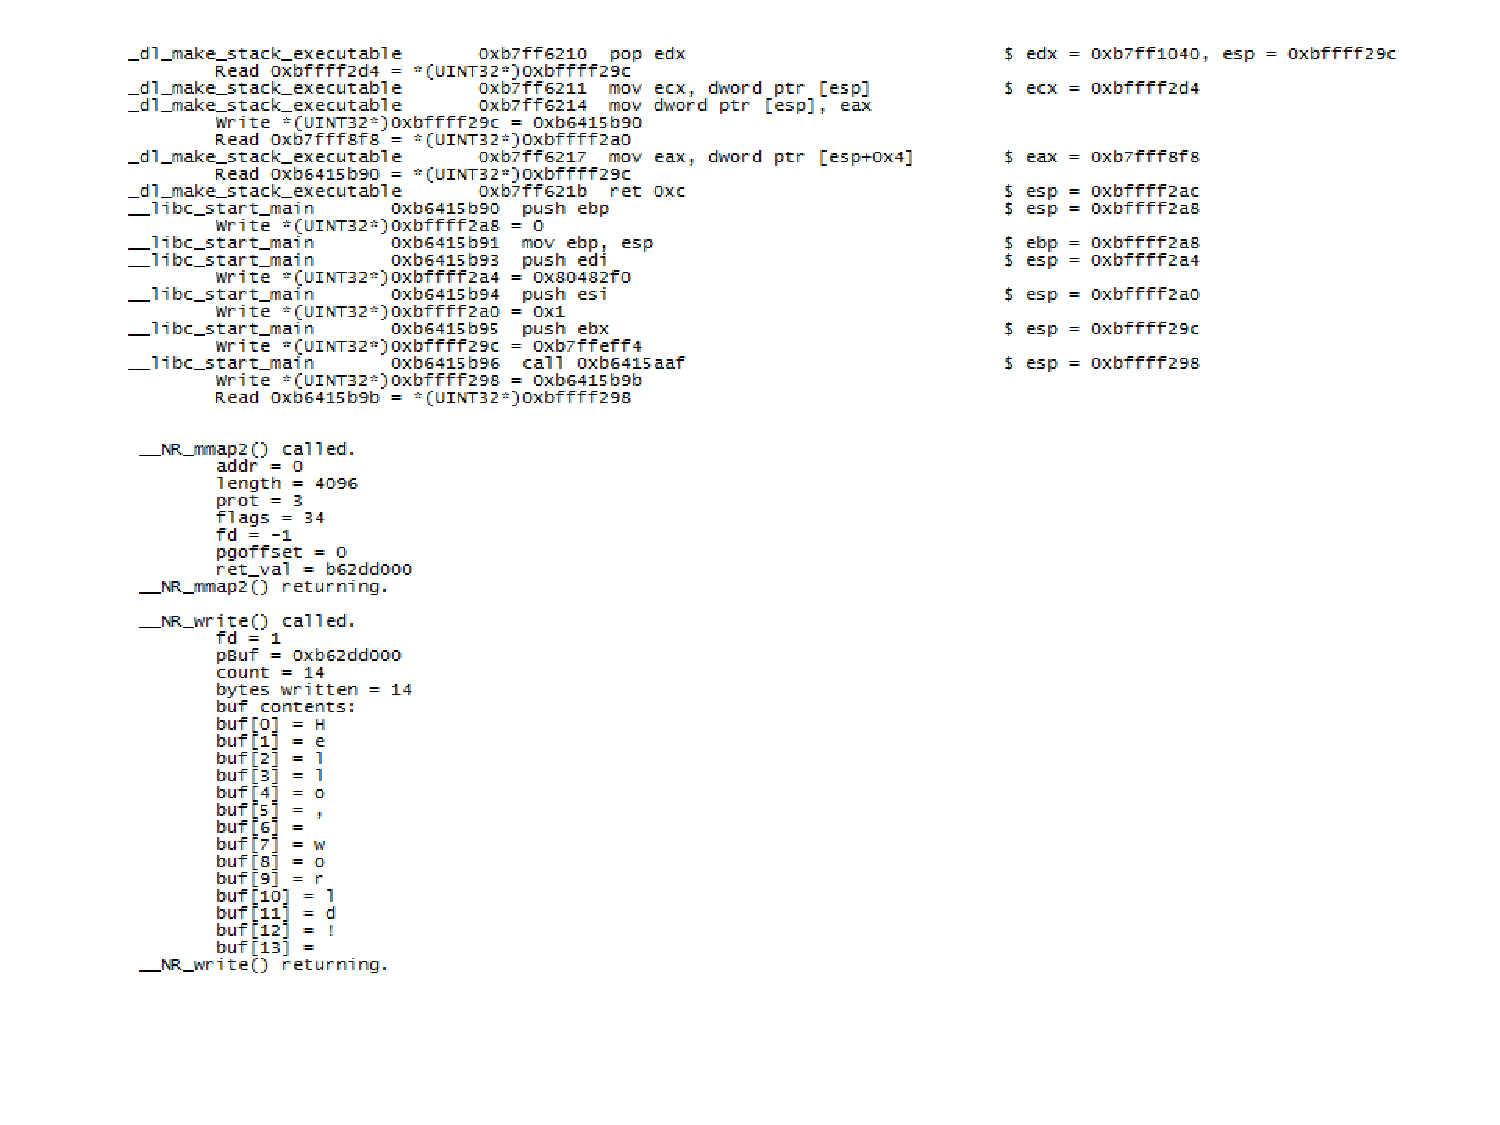
\includegraphics[scale=0.65, trim=2cm 1.5cm 2cm 0.5cm]{log.pdf}
  \caption[An excerpt from the log files generated by the execution tracing layer]%
          {An excerpt from the log files generated by the execution tracing layer.
          The top half shows the set of x86 instructions executed 
          in user-space by the ``Hello, world!'' process, including instruction addresses, 
          symbolic information (wherever available), affected register values and memory 
          addresses. The lower half shows an excerpt from the system call log.}
  \label{hw:logsys}
\end{figure}
\newpage
\noindent {\bf Analysis Script} \newline
The analysis script uses the Linux \emph{diff} utility
to perform pairwise comparisons of the log files generated 
by multiple executions of the target application. 
Using the \texttt{suppress-common}, \texttt{side-by-side}
and \texttt{minimal} flags, the analysis script
produces two output files: 
\begin{enumerate}
\item A {\em delta} file
that contains only instructions that were 
either conflicting between the two logs or missing in one log, and
\item A {\em union} file that contains all instructions
executed in the two logs, but distinguishes instructions  
included in the delta file from matching instructions.
\end{enumerate}
Figure \ref{hw:logsys2} shows an excerpt from the 
union and delta files generated for the ``Hello, world!''
program. These generated files can be used to
detect and diagnose sources of nondeterminism
in an application. The delta and union
files can be constructed from the two
executions that are the most or least different, 
or have the median difference from the set of
collected traces. 

\begin{figure}[h]
  \center
  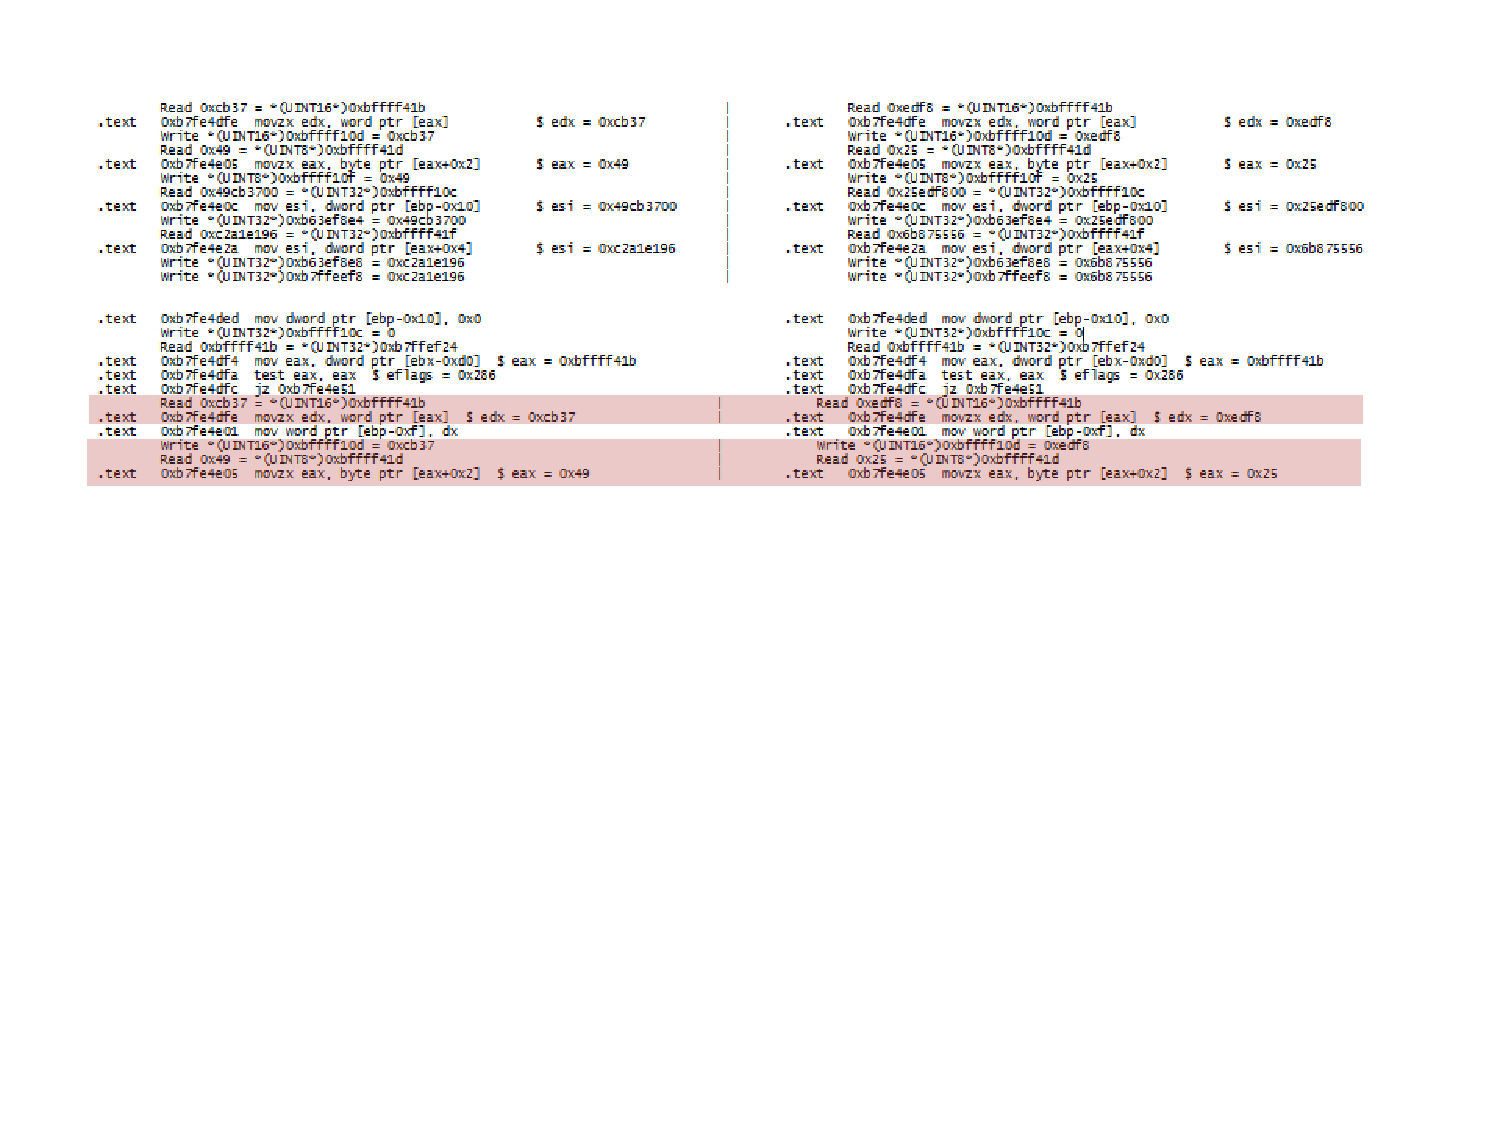
\includegraphics[scale=0.65, trim=2cm 10cm 2cm 0cm]{log2.pdf}
  \caption[Excerpts from the side-by-side diff files generated by the analysis script]%
          {Excerpts from the side-by-side diff files generated by the analysis script.
            The top half shows a few instructions at the start of the delta file;
            these instructions are different in the two logs (as
            indicated by the $\vert$ in the middle of the line).
            The bottom half shows the corresponding instructions in the union file.
            Conflicting instructions are marked with the color red in the 
            union file (along with the $\vert$ symbol); the other instructions are found in both logs.}
  \label{hw:logsys2}
\end{figure}

\newpage
\noindent {\bf Visualization Script} \newline
The visualization script reads the ``union'' file to 
derive statistics on the extent of differences in the
original logs, and generates a diagram to 
capture the different execution traces of the program.
 
In particular, it derives three key metrics
from the ``union'' file:
\begin{enumerate}
\item {\em Length of Common Prefix {\bf (P):}} This is 
the number of instructions common
to both logs starting from the beginning
and up to the point of first divergence.
\item {\em Longest Common Substring {\bf (LS):}}
This is the largest sequence of adjacent instructions 
that are common to both logs.
\item {\em Longest Common Subsequence {\bf (LCS):}}
Intuitively, this is the ``overlap'' in the logs;
it is the length of the longest sequence of instructions
found in both logs. Instructions in the LCS must be in the same order
in both logs, but they are not required to be adjacent.
\end{enumerate}

For instance, if the first instance of a program
executes the instruction sequence $I_1 = [A, B, C, D, E, F]$,
and the second instance of the same program executes 
the instruction sequence $I_2 = [A, B, X, D, E, F, Y]$,
then: the common prefix is $[A, B]$; the longest
common substring is $[D, E, F]$, and the longest
common subsequence is $[A, B, D, E, F]$. 

In general, the longest common subsequence (LCS) of the two traces is
arguably the most indicative of the extent of determinism
in two executions of a program.
The other two metrics are important 
for evaluating the feasibility of deduplication of execution as
a solution to the boot storm problem. In general,
we want the common prefix (P) and the longest common substring (LS)
of the two logs to be as large as possible to
ensure that concurrently booting VMs do not need to branch
execution or communicate with each other too quickly. This
is further discussed in chapter 6.

For the ``Hello, world!'' program, if ASLR
is enabled, the two logs have very little
overlap ($< 5\%$), and the common
prefix and longest common substring
are on the order of $10$ instructions.
With ASLR disabled, one may 
expect the two traces to look identical (because
of the simplicity of the program), but
there is still some nondeterminism in the 
instruction sequences (see Table \ref{hw:stats}
and Figure \ref{hw:trace}).

\begin{table}
\caption{Execution Statistics of ``Hello, world!'' program}
\label{hw:stats}
\begin{center}
\begin{tabular}{||l|c||}\hline
  Common Prefix & 21.49 percent \\\hline
  Longest Common Substring & 67.70 percent \\\hline
  Longest Common Subsequence & 99.98 percent \\\hline
  Conflicts & 0.02 percent \\\hline
\end{tabular}
\end{center}
\end{table}

The figure
% visualization shows where non-determinism occurs and how bursty it is

\begin{figure}[h]
  \center
  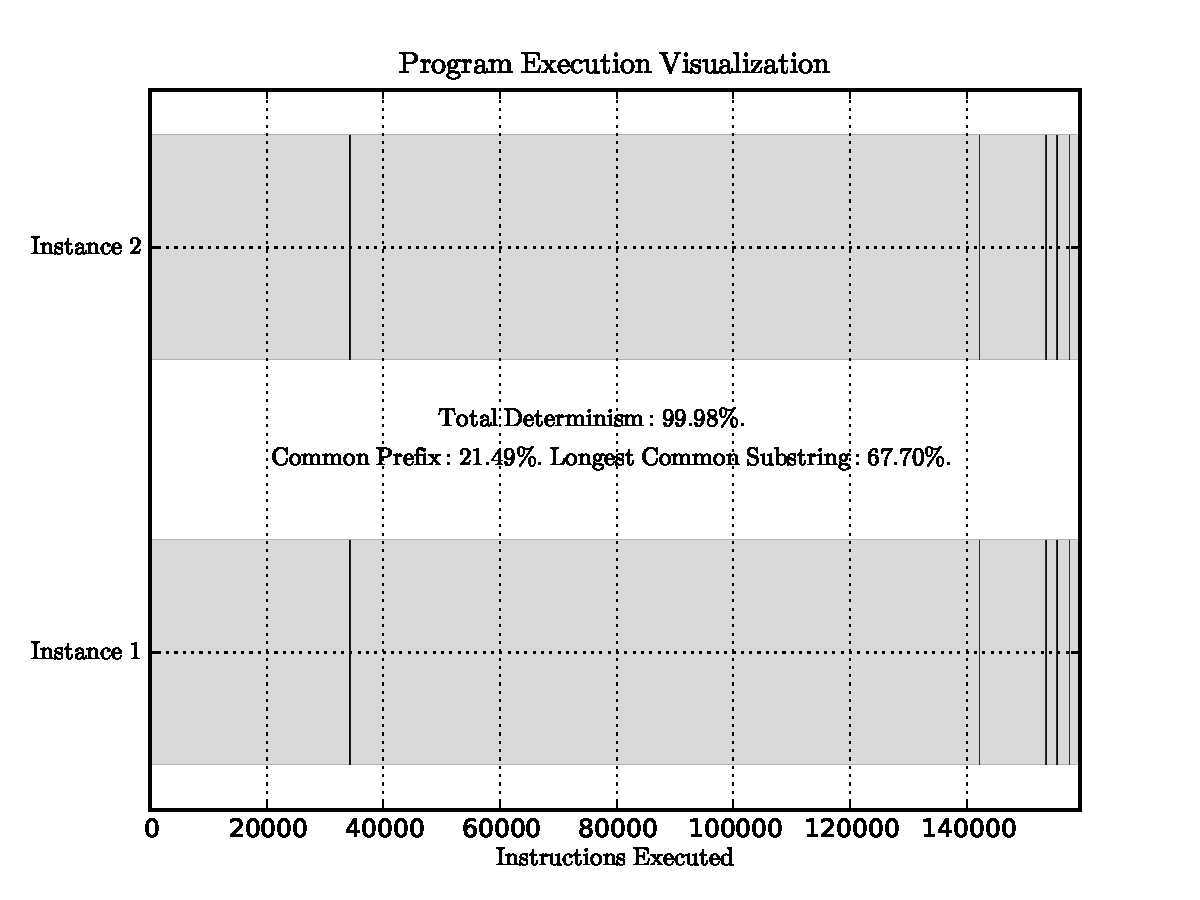
\includegraphics[scale=0.55, trim=0cm 0cm 0cm 0cm]{trace.pdf}
  \caption[Visualization of ``Hello, world!'' program execution]% 
          {Visualization of ``Hello, world!'' program execution.
          The thin black lines represent conflicts between
          the two instances of the program.}
  \label{hw:trace}
\end{figure} 

\section{Statistical Results} \label{bootresults}
% start with helloworld:
% ASLR on -> nothing matches
% introduce notation & diagram
% show results from 3 services:
% visualization (non-determinism is bursty and rare)
% discussion on how image is disproportional but shows importance of nondetermisism

\section{Summary}
